\documentclass{article}
\usepackage{graphicx}
\usepackage{multicol}
\usepackage{hyperref}
\usepackage{a4wide}
\newfont{\normald}{logod10 scaled 1024}
\newfont{\biglogo}{logod10 scaled 2048}
\newcommand{\MF}{{\normald METAFONT}}
\newcommand{\MP}{{\normald METAPOST}}
\newcommand{\FP}{{\normald FEATPOST}}
\newcommand{\AM}{{\normald ANEEMATE}}
\hypersetup{
  pdftitle={Extending MP to 3D and 4D},
  pdfauthor={L. Nobre G.},
  pdfkeywords={MetaPost}
}
\DeclareGraphicsRule{*}{mps}{*}{}
\graphicspath{{../mps/}}
\begin{document}
\title{Extending {\biglogo METAPOST} to 3D and 4D}
\author{L.\ Nobre G.}
\date{\today}
\maketitle
\begin{abstract}
Many authors have been working with three dimensions in \MP\ but, up
to now, these works have not been integrated in the core of \MP. Since
I am one of those authors, I would like to propose now a framing for
that integration. 
\end{abstract}
\setlength{\columnsep}{2.5em}
\begin{multicols}{2}
\tableofcontents
\end{multicols}
Since {\tt colors} and {\tt cmykcolors} were introduced in \MP, it
became a simulation machine. Ordinary differential equations could be
solved in 3D or 4D using the exact same Runge--Kutta code as for 2D.

But some way of projection had to be developed by the user in order to
draw the results of the simulation. 

\section{Projecting from 3D into 2D}

Many different kinds of projections exist, I tried a few and I think
it is enough to project  through a single point $\vec{f}$ onto a 
plane\footnote{When the point is at infinity, the projection is
  parallel and it defines only a direction.}.
This kind of projection can take advantage of \MP's linear equations.
Take, for instance, the following figure.
\begin{center}
  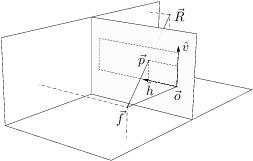
\includegraphics[width=0.6\textwidth]{photorefer.2}
\end{center}
Point $\vec{p}$ can be calculated from the following equations:
\begin{equation}
  \left\{
    \begin{array}[c]{l}
      \vec{R}+\lambda\left(\vec{R}-\vec{f}\right) = \vec{o}+\vec{p} \\
      \left(\vec{h}\times\vec{v}\right)\cdot\vec{p} = 0
    \end{array}
  \right.
\end{equation}
which can be coded as below:
\begin{quote}
\begin{verbatim}
color p;
R + whatever*(R-f) = o + p;
(h crossproduct v) dotproduct p = 0;
\end{verbatim}
\end{quote}
where {\tt R, f, o, h} and {\tt v} are known {\tt colors}. Of course,
this requires that one defines {\tt crossproduct}, the cross product of
two vectors\footnote{I don't know how to define the cross product in
  4D.}.
This kind of projection is called ``perspective'' and can easily
be transformed into a parallel projection, like this:
\begin{quote}
\begin{verbatim}
color p;
R + whatever*(o-f) = o + p;
(h crossproduct v) dotproduct p = 0;
\end{verbatim}
\end{quote}
There are a few problems, though:
\begin{itemize}
\item Depending on the positions of $\vec{f}$ and $\vec{R}$ the linear
equations may produce divisions by zero. But these equations are quite
simple and can be solved in advance so that divisions by zero can be
caught as is done in \FP.
\item $\vec{p}$ is a {\tt color}, not a {\tt pair}, so it must be
converted. But this is very easy:
\begin{quote}
\begin{verbatim}
x = p dotproduct h;
y = p dotproduct v;
\end{verbatim}
\end{quote}
\item if both $\vec{R}$ is a node or control point of a 3D path and
  the projection is a perspective then the path perspective is no
  longer a B\'{e}zier spline, it is a non-uniform rational basis spline
  (NURBS). The only way around this is to ignore the problem.  
\end{itemize}

\subsection{Exactly how?}
 
Given that the actual way to draw a 3D path depends not only on the
definition of that path but also on the kind of projection being used,
I propose that the projection be done only at {\tt shipout} time.

A perspective is not an affine transform and cannot be inverted by
linear equations. A perspective is a new thing for \MP. 

The parallel projection is an affine transform but \MP\ has not yet a
framework neither for 3D nor for 4D {\tt transforms}.

The transition from the actual \MP\ to a full--fledged 3D \MP\ depends
critically on the support for smooth 3D and 4D paths. 

Once \MP\ is beyond this
transition what will certainly show up is the need for full path
tansforms which may either be affine or not. I propose to call these
``generic'' transforms as {\tt maps}. But note that these full path
transforms cannot be perspectives because they only map each node and
control point of a given path\footnote{A {\tt map} may be regarded as
  an approximation of a perspective.}. 

\section{The whole package}

\subsection{Already on the Tracker}

The next most basic 3D and 4D capability that needs to be added to
\MP\ is already published as Tracker item \# 104: both {\tt abs} and
{\tt unitvector} must be expanded to accept {\tt colors} and {\tt
  cmykcolors} as arguments.

\subsection{Cross product}

A good {\tt crossproduct} for \MP\ would accept {\tt numerics}, {\tt
  pairs} and {\tt colors} as arguments.
\begin{description}
  \item[{\tt numerics}] the result is {\tt 0}
  \item[{\tt  pairs A} and {\tt B}] the result is a {\tt color} with
    all parts null except that the {\tt bluepart=Ax*By-Ay*Bx}
  \item[{\tt colors}] the result is the standard cross product
\end{description}

\subsection{\tt angle}

\begin{quote}
\begin{verbatim}
color A, B;
angle( A, B ) = angle( abs( A crossproduct B ), A dotproduct B );
\end{verbatim}
\end{quote}

\subsection{Commands to be adapted}

The following commands should be adapted to accept 3D (and 4D) points and
paths:
\begin{quote}
\begin{verbatim}
draw undraw drawarrow drawdblarrow
fill unfill filldraw unfilldraw
reverse
precontrol postcontrol
arclength arctime
label dotlabel
slanted shifted rotated scaled xscaled yscaled 
rotatedaround reflectedabout
bbox
subpath
path
transform transformed identity inverse
direction of
point of
\end{verbatim}
\end{quote}
And the following commands should be adapted to accept the new 3D and
4D {\tt transforms}
\begin{quote}
\begin{verbatim}
xpart ypart xxpart xypart yxpart yypart
cyanpart magentapart yellowpart blackpart
\end{verbatim}
\end{quote}
%%%%%%%           $$ \hbox{\verb|draw (20,20)--(0,0)|} $$

\subsection{New commands}

{\tt Colors} and {\tt cmykcolors} should have analogues to {\tt z} to
be wiped--out on {\tt beginfig}. I propose {\tt C} for {\tt colors}
and {\tt D} for {\tt cmykcolors}. There should exist predefined names for
unitary 4D vectors like {\tt purecyan = (1,0,0,0); puremagenta =
  (0,1,0,0)}, etc. 
\begin{quote}
\begin{verbatim}
zscaled tdtransform tdtransformed fdtransform fdtransformed
xzpart yzpart zzpart zpart zxpart zypart
ccpart cmpart cepart ckpart
mcpart mmpart mepart mkpart
ecpart empart eepart ekpart
kcpart kmpart kepart kkpart
mapped
\end{verbatim}
\end{quote}
This last one {\tt mapped} is perhaps the most messy of all. It should
work like this:
\begin{quote}
\begin{verbatim}
anypath mapped NameOfUserMap;
\end{verbatim}
\end{quote}
where {\tt NameOfUserMap} is the name of a macro that uses as a single
argument each node and control point of the {\tt anypath}. It returns
a new path that may have different dimensionality\footnote{Standard
  affine {\tt transforms} keep the dimensionality.} 

\subsection{Commands that should not be touched}

One of the problems of extending \MP\ is that somethings really cannot
be extended. This is related with the smoothness of 2D paths. With the
exception of cusp points, the {\tt direction} is well--behaved on a 2D
path. But on a 3D path (and specially on a 4D path) most directions
cannot be found. Also, {\tt intersections} become exceedingly hard to
find. 

\end{document}